\documentclass{article}

\usepackage{color}
\usepackage{tikz}
\usepackage{float}
\usepackage{tabularx}
\usepackage{amsmath}
\usepackage{amssymb}
\usepackage{listings}
\usepackage{enumitem}
\usepackage{syntax}
\usepackage{csquotes}
\usepackage{pgfplots}
\usepackage{parskip}
\usepackage{fancyhdr}
\usepackage{vmargin}
%\usepackage[backend=biber]{biblatex}
%\addbibresource{references.bib}


\definecolor{dkgreen}{rgb}{0,0.6,0}
\definecolor{gray}{rgb}{0.5,0.5,0.5}
\definecolor{mauve}{rgb}{0.58,0,0.82}

% Plots
\usepackage{pgfplots}
\usepackage{pgfplotstable}
\pgfplotsset{filter discard warning=false}
\pgfplotsset{
    discard if/.style 2 args={
        x filter/.append code={
            \edef\tempa{\thisrow{#1}}
            \edef\tempb{#2}
            \ifx\tempa\tempb
                \def\pgfmathresult{inf}
            \fi
        }
    },
    discard if not/.style 2 args={
        x filter/.append code={
            \edef\tempa{\thisrow{#1}}
            \edef\tempb{#2}
            \ifx\tempa\tempb
            \else
                \def\pgfmathresult{inf}
            \fi
        }
    },
    discard if smaller/.style n args={2}{
    	x filter/.code={
            \edef\tempa{\thisrow{#1}}
            \edef\tempb{#2}
                \ifnum\tempa<\tempb
                    \def\pgfmathresult{inf}
                \else
                \fi
        }
    },
    discard if larger/.style n args={2}{
    	x filter/.code={
            \edef\tempa{\thisrow{#1}}
            \edef\tempb{#2}
                \ifnum\tempa>\tempb
                    \def\pgfmathresult{inf}
                \else
                \fi
        }
    }
}


% Listings
\usepackage{algorithm}
\usepackage[noend]{algpseudocode}

\lstset{frame=tb,
  numbers=left,
  stepnumber=1,
  language=Java,
  aboveskip=3mm,
  belowskip=3mm,
  showstringspaces=false,
  columns=flexible,
  basicstyle={\small\ttfamily},
  numberstyle=\color{gray},
  keywordstyle=\color{blue},
  commentstyle=\color{dkgreen},
  stringstyle=\color{mauve},
  breaklines=true,
  breakatwhitespace=true,
  tabsize=2,
  moredelim=**[is][\color{red}]{@}{@},
}

\setlength{\grammarindent}{12em}

%\renewcommand{\lstlistingname}{Algorithm}
%\newcommand{\tablerow}[4]{ #1 & #2 & #3 & #4\\}
\newcommand{\n}[0]{\\[\baselineskip]}

% TITLE PAGE
% #1 - Module code
% #2 - Lecturer
\newcommand{\maketitlepage}[2]{
\begin{titlepage}
	\centering
    
\includegraphics[scale = 0.4]{imgs/logo.png}\\	% University Logo
	\textsc{\LARGE #1}\\[0.5 cm]				% Course Code
	\rule{\linewidth}{0.2 mm} \\[0.4 cm]
	{ \huge \bfseries \thetitle}
	\rule{\linewidth}{0.2 mm} \\[0.5 cm]
	\textsc{\large \thedate}\\[1.5 cm]
	
	\begin{minipage}{0.4\textwidth}
		\begin{flushleft} \large
			\emph{Lecturer:}\\
			#2
			\end{flushleft}
			\end{minipage}~
			\begin{minipage}{0.4\textwidth}
            
			\begin{flushright} \large
			\emph{Submitted By:} \\
			\theauthor
		\end{flushright}
        
	\end{minipage}\\[2 cm]
	
\end{titlepage}
}




\title{Classification of object colour using optical spectroscopy}
\author{140011146}

\makeatletter
\let\thetitle\@title
\let\theauthor\@author
\let\thedate\@date
\makeatother

\begin{document}

\maketitlepage{CS5014 Machine Learning}{David Harris-Birtill\\Kasim Terzi\'{c}}



\section{Introduction}

In this practical, two classification tasks were performed on an experimental dataset. The classification task was to identify different colours from spectroscopy data. The first task was a binary classification task with only two colours and the second was an extension to the binary task with the introduction of additional colours. 

\section{Binary Classification}

\subsection{Preprocessing}
Before any preprocessing is done, the data was split into training and test datasets. This is to ensure no bias when looking at the data, even for visualisations. The split is also stratified over the output to ensure the training and test sets have the same proportion of classes that is found in the original data. This again is done to prevent bias and overfitting as much as possible so that the trained model is not overfit to a subset of the data with a different proportion of classes. 
\n
Nothing was done about the negative intensities found in the data as this came from issues during data collection where the distance of the spectrometer changed. It is not trivial to account for the errors as the distance moved is not known. Further, scaling to the negative values to keep the intensities going from 0-100\% is likely to skew the data in an unknown way. Removing all data points where negative values exist would also hurt as the dataset is already quite small. Because of these reasons, the data was not cleaned for negative intensities. Furthermore the data was not normalised. This is because all the input features represented the same units of measurement and so there is not any difference between the ranges of each feature. 


\subsubsection{Data visualisation}
First, the spectroscopy data can be visualised by plotting the intensities and wavelengths to see if there are visual patterns than can be seen in the data. As there are over nine hundred input features, it is likely many of them are either redundant or not well correlated to the input data. 

\begin{figure}[H]
\centering
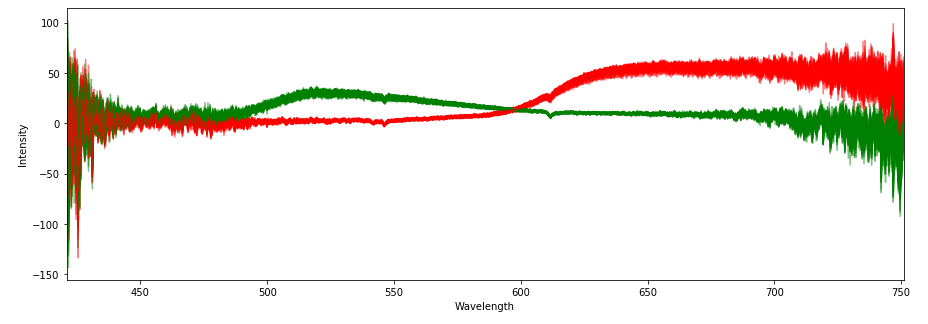
\includegraphics[width=1\textwidth, keepaspectratio]{imgs/binary-visual.png}
\caption{Initial plot of the data, showing the intensity of the wavelengths measured. The plot is colour coded with the output so any differences between the red and green data can be easily seen.}
\label{fig:binary-visual}
\end{figure}
\noindent
From the visualisation, it is interesting to see that for many wavelengths, there is a very clear distinction between the red and green intensities. This suggests that for those wavelengths, it would be very simple to classify. Further, the visualisation was created from all the training data, so it can be seen there are no large errors in the middle wavelengths where no data points incurred significant differences, which shows the consistency of the data. It can be see towards the start and end of the spectrum, the intensities are more varied, indicating possible errors during measurement. As such, it would make sense when choosing input features to mostly include features from the middle wavelengths where less possible errors occurred. 

\subsubsection{Data correlation}
Next, the correlation of each input feature wavelength can be calculated and plotted to see how the set of input features is correlated to the output. It is not feasible to plot each input feature's correlation separately due to the large number of features. Therefore all the features are put onto the same graph for comparison.
\begin{figure}[H]
\centering
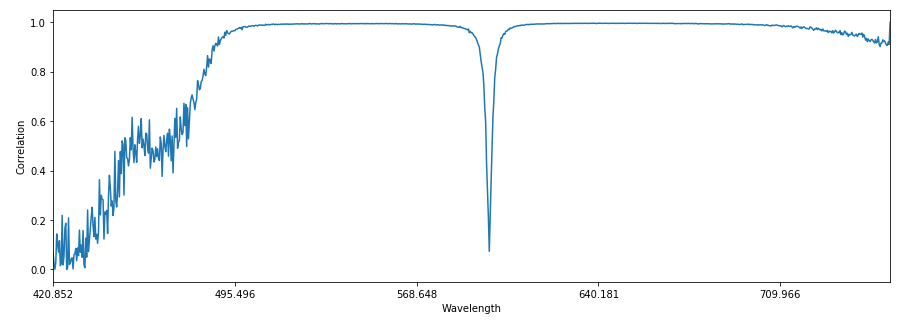
\includegraphics[width=1\textwidth, keepaspectratio]{imgs/binary-correlation.png}
\caption{Correlation of each wavelength input feature to the output classification.}
\label{fig:binary-correlation}
\end{figure}
\noindent
The curve of input feature correlation corresponds very closely to figure \ref{fig:binary-visual}. At the beginning where there seems to be more noise, the correlation is low. At the wavelengths where the red and green curves start to become distinct from each other, the correlation of that wavelength to the output class tends to perfect correlation. At the center where the red and green curves cross over, a dip in the correlation can be seen as it becomes difficult to distinguish the two in the overlap. This is good news and expected, as the clear difference between the red and green curves corresponds to a clear classification. 
\n
To show this more clearly, the histograms of a single input feature can be visualised.

\begin{figure}[H]
\centering
\subfigureimage{0.45\textwidth}
{imgs/binary-onefeaturebad.png}
{Histogram of a wavelength where there is high overlap and low correlation between the red and green curves.}
\hspace*{\fill}
\subfigureimage
{0.45\textwidth}
{imgs/binary-onefeaturegood.png}
{Histogram of a wavelength where the red and green curves are distinct and there is perfect correlation with the output class.}

\caption{Comparison of histograms of a single wavelength measurement. One taken at a low correlation wavelength and the other at a high correlation wavelength.}
\label{fig:binary-histogram-comparison}
\end{figure}
\noindent
The histograms in figure \ref{fig:binary-histogram-comparison} show the difference between an input feature with low correlation and an input feature with high correlation. The two wavelengths were arbitrarily chosen based on the correlation graph, but an obvious difference can still be seen. With low correlation, there is a lot of overlap between the two classes, which could also have been seen in figure \ref{fig:binary-visual}. For  the input feature with high correlation, the histogram shows very clearly the separation between the two classes. Figure \ref{fig:binary-histogram-more} further supports the fact that all input feature wavelengths where the correlation is high and a clear distinction seen in figure \ref{fig:binary-visual} have clear, separate intensities. As the histograms contain all data points from the split training set, it is very likely that a single input feature can lead to a high classification rate. 

\begin{figure}[H]
\subfigureimage{0.31\textwidth}
{imgs/binary-onefeature1.png}
{Wavelength 495.496}
\hspace*{\fill}
\subfigureimage{0.31\textwidth}
{imgs/binary-onefeature2.png}
{Wavelength 640.181}
\hspace*{\fill}
\subfigureimage{0.31\textwidth}
{imgs/binary-onefeature3.png}
{Wavelength 709.966}
\caption{Further histograms of highly correlated wavelengths, showing the separation of the two classes occurs for many different input features.}
\label{fig:binary-histogram-more}
\end{figure}



\subsection{Results}
From the preprocessing stage, it was shown that there are multiple input features where a clear distinction using just that single input feature could be seen between the two classes. As such, a single input feature is tried first for training to see what classification rates could be obtained. 
\begin{table}[H]
\centering
\begin{tabular}{| c | c |}
\hline
\textbf{Input feature} & \textbf{Accuracy} \\
\hline
Wavelength 421.228 & 0.5 \\
\hline
Wavelength 495.496 & 1.0 \\
\hline
Wavelength 568.648 & 1.0 \\
\hline
Wavelength 640.181 & 1.0 \\
\hline
Wavelength 709.966 & 1.0 \\
\hline
\end{tabular}
\caption{Results of training a logistic regression model on a single input feature.}
\end{table}
\noindent
Despite the indications that the data would be easy to classify, the predictions from the logistic regression model are suspiciously high. All single input features used that had a high correlation gave perfect accuracy during prediction. The first thought was that perhaps the model is overfitting, so the same training is done again with k-fold cross validation. 
\begin{table}[H]
\centering
\begin{tabular}{| c | c | c | c |}
\hline
\textbf{Input feature} & \textbf{5 fold accuracy} & \textbf{10 fold accuracy} & \textbf{25 fold accuracy} \\
\hline
Wavelength 421.228 & 0.5 & 0.49 & 0.5 \\
\hline
Wavelength 495.496 & 1.0 & 1.0 & 1.0 \\
\hline
Wavelength 568.648 & 1.0 & 1.0 & 1.0 \\
\hline
Wavelength 640.181 & 1.0 & 1.0 & 1.0 \\
\hline
Wavelength 709.966 & 1.0 & 1.0 & 1.0 \\
\hline
\end{tabular}
\caption{Accuracy of using k-fold cross validation to show the logistic regression model is not overfitting.}
\end{table}
\noindent
Even with using a high k-fold cross validation, the strong input features continued to get 100\% accuracy, showing it is unlikely due to overfitting but because the data and those specific input features lends themselves well to a binary classification. It was further confirmed how well defined the classification was by splitting the training data into an even smaller dataset with only 10\% of the training dataset used for training and testing on the rest of the training data. Here there is a slight discrepancy between  training and testing accuracy where certain input features obtained slightly lower accuracy when running on the test data. This tells us that even with a very well defined classes as seen from previous training models and visualisations, it is difficult for models to generalise well given very few samples. At the same time, the fact that such a high testing accuracy could still be obtained from such a low number of training samples once again shows the clear difference between the classes.

\begin{table}[H]
\centering
\begin{tabular}{| c | c | c |}
\hline
\textbf{Input feature} & \textbf{Training accuracy} & \textbf{Testing accuracy}\\
\hline
Wavelength 421.228 & 0.67 & 0.46\\
\hline
Wavelength 495.496 & 1.0 & 0.98\\
\hline
Wavelength 568.648 & 1.0 & 0.99\\
\hline
Wavelength 640.181 & 1.0 & 1.0\\
\hline
Wavelength 709.966 & 1.0 & 1.0\\
\hline
\end{tabular}
\caption{Accuracy of training logistic regression on 10\% of the training data and testing on the remaining 90\%.}
\end{table}
Three more approaches were used as a final way of checking that one input feature is enough for a good classification of this problem. First the accuracies of each single input feature is calculated by training a logistic regression model with that feature and plotting the accuracies. Next, recursive feature elimination was used to get the accuracy score as the number of features used increased to show any more than two input features will always give 100\% accuracy. Recursive feature elimination is a method of recursively selecting smaller and smaller number of features. On each recursive step, the given model is trained on a set of features, then the features deemed least important are removed. This is done until a specified number of features is reached. Finally, a decision tree classifier was used to verify both the 100\% accuracy and one input feature being enough.
\begin{figure}[H]
\centering
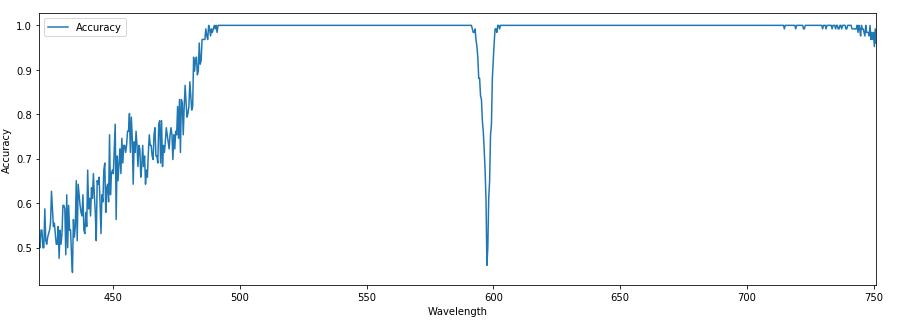
\includegraphics[width=1\textwidth]{imgs/binary-accuracy.png}
\caption{All input feature wavelengths trained individually and their accuracies graphed.}
\label{fig:binary-accuracy}
\end{figure}
%
\begin{figure}[H]
\centering
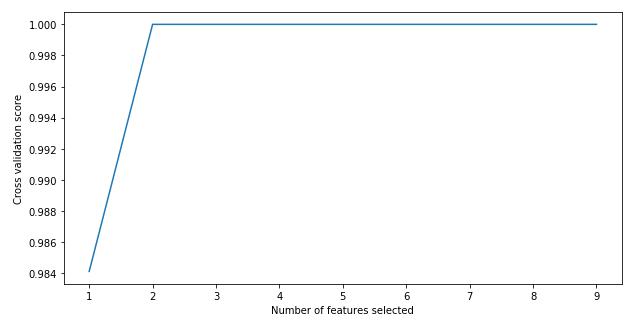
\includegraphics[width=0.7\textwidth, keepaspectratio]{imgs/binary-numfeatures.png}
\caption{Cross validation accuracy score of increasing number of features using recursive feature elimination.}
\label{fig:binary-accuracyrfecv}
\end{figure}
\noindent
Figure \ref{fig:binary-accuracy} shows the accuracy of each input feature when used alone to train the logistic regression model. It can be seen to be very similar to figure \ref{fig:binary-correlation} which showed the correlation of each input feature. This indicates the well correlated features are also the ones that have good accuracies with little noise disrupting this pattern. The graph of accuracy obtain from recursive feature elimination with cross validation does not confirm it is always the case the one input feature is enough for perfect classification. This is because of the wavelengths at the beginning and end of the data where there is more overlap. However, one input feature already gets a 0.992 classification rate on average and any more than one feature always gets 100\%. 
\n
Finally, a decision tree classifier was used to confirm the high accuracy as well as see that a single input feature was enough for this task. A decision tree was used because it uses learns simple decision rules and if only one feature was needed, then the decision tree will show it clearly as a single depth needed in the tree and this can be visualised. 
\begin{figure}[H]
\centering
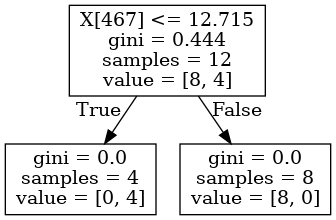
\includegraphics[width=0.4\textwidth, keepaspectratio]{imgs/binary-decisiontree.png}
\caption{Decision tree classifier showing only one decision needed for binary classification}
\end{figure}
\noindent
The decision tree for binary classification shows that only one input feature is needed to make the decision to classify between the two colours. When run multiple times, the exact input feature used (\texttt{X[467]}) changes, showing there are multiple single input features that could be used. Furthermore, the decision tree was also able to get 100\% accuracy training on the small  10\% reduced set and testing on the other 90\%. 

\subsection{Evaluation}
From the initial visualisations of the binary classification data, it could be seen that for a range of wavelengths, the two classes of red and green colours were easily distinguishable by eye. This was further confirmed by graphing the correlation of each wavelength to the output classification and shown clearly by plotting the histogram of a single wavelength, which showed a clear separation between the classes. Because of these observations, it was not a huge surprise that a simple logistic regression model was able to perform perfect classification on the training data, using specific single input features. The results were confirmed to not be due to overfitting, as k-fold validation was performed with a large value of k. Moreover, it was shown that with a training set size of just 10\% (12 data points), the high classification rate was still retained when predicting the other 90\% (114 data points).
\n
The results make sense when coming back to what the actual classification problem is. The data represents spectroscopy data with red and green colours placed under the device. As red and green are very distinct colours with different wavelengths, it was natural that there would be a clear separation between the colours.
\n
Because of the high accuracy obtained by the logistic regression model, no further machine learning models were used or tried on the dataset except for the decision tree classifier to verify the results from logistic regression. This was done for a few reasons. First, little improvement in terms of accuracy could be gain from using different models if the accuracy from logistic regression is already at 100\% using one input feature and 12 training data points, so there is little point to try and optimise further. Second, most other machine learning models involved more complexity than a logistic regression model so if little improvement can be made, it seemed more practical to stick with the simple model rather than try something more complex, which would naturally take a longer time to run if the dataset was extremely large. 

\section{Multiclass Classification}
For the multiclass classification, many of the same steps as the binary task were taken. Because of the added complexity of more classes, the results were not the same and hence the steps deviate from the binary task at a certain point. It is reasonable to use knowledge gained from the binary classification task and apply it to this multiclass task because the problem is the same. The input features are exactly the same as in the binary task, the difference being there are more classes and as a result more data points. Hence, some of the knowledge gained before can be used here to inform some decisions. 

\subsection{Preprocessing}
Again the data was split into training and test data at the very beginning before any further visualisation or analysis. Stratification was also used on the output to ensure the same proportion of classes in both the training set and testing set. Additionally, the data was not cleaned or normalised for the same reasoning explained for the binary classification.
\subsubsection{Data visualisation}
With the additional colour classes in the dataset, it can be seen that there are more areas of overlap and no clear wavelengths where all colours are distinct from each other. The pattern of having noisy input at the early and late wavelengths is still apparent in this data, which shows the measurement was relatively consistent to the data for binary classification. Because of the additional colours, it may be expected that a single input feature would not be enough to classify the colours. Particularly the pink and red wavelength intensities look like they follow a very similar pattern, which makes sense as they are the closest colours out of the five. These two colours may be one of the more difficult to determine between compared to the other classes.
\begin{figure}[H]
\centering
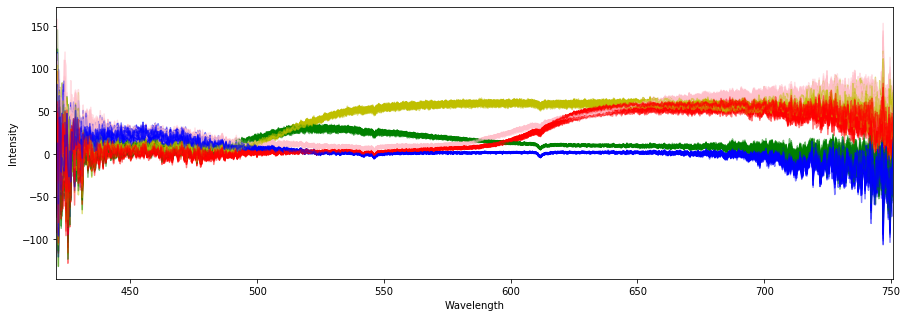
\includegraphics[width=1\textwidth, keepaspectratio]{imgs/multiclass-visual.png}
\caption{Plot of the data to show the intensity of wavelengths of the different colour classes.}
\label{fig:multiclass-visualisation}
\end{figure}

\subsubsection{Data correlation}
The correlation of each input feature to the output class is graphed to see if similar patterns as the binary classification can be seen.
\begin{figure}[H]
\centering
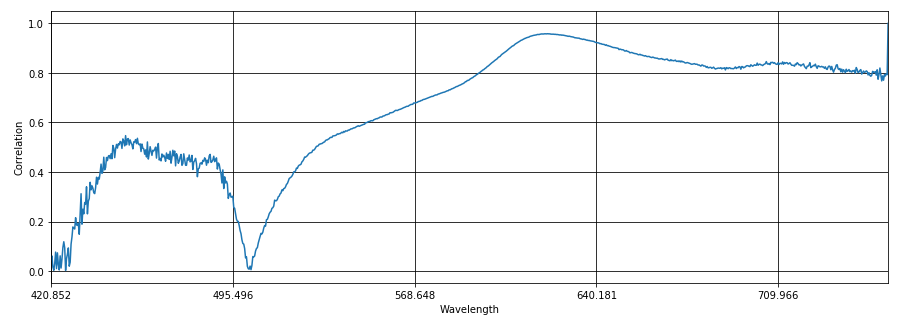
\includegraphics[width=1\textwidth, keepaspectratio]{imgs/multiclass-correlation.png}
\caption{Correlation of each wavelength input feature to the colour classification.}
\end{figure}
\noindent
Unlike in binary classification, here there is never a single input feature where there is perfect correlation and this follows from the visualisation of the data in figure \ref{fig:multiclass-visualisation}. Some ranges of wavelengths have a high correlation than others, but not enough to completely classify each of the five classes. To get a good idea of how the data is spread for each wavelength, a few histograms are created like in the binary task.
\begin{figure}[H]
\centering
\subfigureimage{0.31\textwidth}
{imgs/multiclass-onefeature1.png}
{Wavelength 420.852}
\hspace*{\fill}
\subfigureimage{0.31\textwidth}
{imgs/multiclass-onefeature2.png}
{Wavelength 495.496}
\hspace*{\fill}
\subfigureimage{0.31\textwidth}
{imgs/multiclass-onefeature3.png}
{Wavelength 568.648}

\vspace{0.5cm}

\subfigureimage{0.31\textwidth}
{imgs/multiclass-onefeature4.png}
{Wavelength 604.625}
\hspace*{\fill}
\subfigureimage{0.31\textwidth}
{imgs/multiclass-onefeature5.png}
{Wavelength 640.181}
\hspace*{\fill}
\subfigureimage{0.31\textwidth}
{imgs/multiclass-onefeature6.png}
{Wavelength 709.966}
\caption{Histograms of single input features for multiclass classification}
\end{figure}
\noindent
Because of the additional classes, there is a much less clear distinction between all the colours. For example we can see for wavelength of 420nm, 495nm and 709nm there is significant overlap between at least two classes. The intensities at wavelength 568nm and 604nm show a clearer difference, but there is not a large margin of difference between some classes, for example red and pink. This suggests that one input feature is not likely to be enough to get perfect classification like in the binary case. Further, models could be more prone to overfitting, as the lack of large margin difference in a single input feature means any small outliers may cross into another class boundary more easily. With more than a single input feature, the combination of different boundaries for different wavelengths could uniquely identify the class. 

\subsection{Results}
To get an idea of the optimal number of input features that should be used, recursive feature elimination is used. A logistic regression model is used first following the good results this simple model got during the binary classification task. From the scikit-learn library, applying a logistic regression model uses a one-vs-all method method.

\begin{figure}[H]
\centering
\subfigureimage{0.48\textwidth}
{imgs/multiclass-numfeatures1.png}
{Showing all features}
\hspace*{\fill}
\subfigureimage{0.48\textwidth}
{imgs/multiclass-numfeatures2.png}
{Showing only up to 15 features}
\caption{Cross validation accuracy score of increasing number of features with recursive feature elimination for multiclass classification.}
\end{figure}
\noindent
It can be seen there is an odd dip at the beginning when using fewer features. Upon closer inspection, at three and four input features the accuracy becomes 100\%, but dips back down from including more features before going back to 100\% after thirteen features. This suggests that between five and twelve input features, the addition of more features sometimes causes noise that is not well correlated to other features, causing some overfitting. As the logistic regression model uses one-vs-all, this means that for the additional features (wavelengths) added, each colour is not completely distinct from all the other colours. It should be noted that the dip is a \textit{very} small dip in accuracy, from 100\% to 99.67\%. Past twelve features, the accuracy stays at 100\% up to using all features from the data. This shows that with enough wavelength information, it is possible to always classify the different colours. Adding additional features does not lead to overfitting in this case because there is little noise in the actual data and all the input features represent the same thing in wavelength intensity, so it does not become the case that having all the input features adds irrelevant information, but more the case it simply adds redundant information. 
\n
As it is expected using all the input features would get 100\% accuracy, the goal pursued was to see the kind of accuracies that could be gained with as few features as possible. From the visualisations earlier, it may be possible with one feature, but fewer features may also make the model harder to generalise, especially with less training data. 
\begin{table}[H]
\centering
\begin{tabular}{| c | c |}
\hline
\textbf{No. of input features} & \textbf{Training acc.} \\
\hline
1 & 0.73 \\
\hline
2 & 1.0 \\
\hline
3 & 1.0 \\
\hline
4 & 1.0 \\
\hline
\end{tabular}
\caption{Accuracy of training with different number of input features for multiclass classification.}
\end{table} 
From training on all the data from the training set, it was possible to get 100\% accuracy with 2 features. Again, we must do more to ensure this is not a case of overfitting. Both cross validation and training with significantly less sample points were done like in binary classification to confirm any absence of overfitting and to show that the model can generalise to larger volumes of unseen data with few features and few training examples. 
\begin{table}[H]
\centering
\begin{tabular}{| c | c | c | c |}
\hline
\textbf{No. of input features} & \textbf{10 fold acc.} & \textbf{50 fold acc.} & \textbf{10\% training size test acc.} \\
\hline
1 & 0.727 & 0.721 & 0.581 \\
\hline
2 & 1.0 & 0.998 & 0.996 \\
\hline
3 & 1.0 & 1.0 & 1.0 \\
\hline
4 & 1.0 & 1.0 & 0.993 \\
\hline
\end{tabular}
\end{table}
\noindent
It can be seen that similar to the case with binary classification, where 100\% accuracy could be obtained from training on all the training data, using additional methods confirms the fact that the result is not a case of overfitting. There is only a very small drop in accuracy from using a large k-fold validation and from using a small 10\% training size. It is interesting to see that with 3 input features, no loss of accuracy can be seen despite the methods used, showing the logistic regression model with 3 input features is able to generalise very well to unseen data. 
\n
As it seemed a small number of input features was needed, a decision tree was used again to confirm and visualise this. 
\begin{figure}[H]
\centering
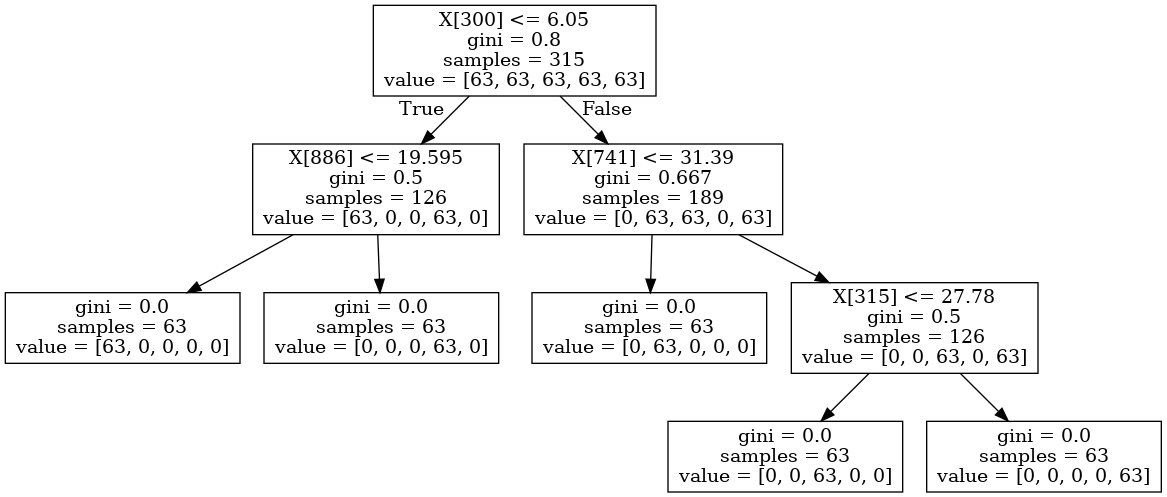
\includegraphics[width=0.9\textwidth, keepaspectratio]{imgs/multiclass-decisiontree.png}
\caption{Decision tree showing 4 input features needed for multiclass classification.}
\end{figure}
\noindent
The decision tree classifier needed 4 different wavelengths to classify the colours and also got 100\% accuracy. It can be seen that with the 4 features, the different colours are very clear split after each decision, with no samples of different classes overlapping into other nodes, once again confirming the ease of classification of this problem. 

\subsection{Evaluation}
Many of the results and methods used for multiclass classification were very similar to the binary classification problem. This was to be expected to some extent, as the multiclass problem was a direct extension of the binary problem to more classes. However, what was not expected was the high classification rate and good results gained from using the same simple methods as binary classification. The possibility that the logistic regression model was overfitting was explored thoroughly through the use of cross validation and training with a very small sample size to show it was not an issue. 

Because the multiclass extension requires classification of more colours, it was thought that more sophisticated models may have been needed. In the end, it was shown that to be able to extend a binary colour classification to a multi-colour classification, a logistic regression classifier with one-vs-all method with additional wavelengths as input features was all that was needed to be able to uniquely identify more colours. This result is interesting, as it shows this problem of colour classification could be easily extensible to even more colours by applying more wavelengths as input features. This also shows how the wavelengths are a very well correlated feature to the colour of an object and so it is possible to extend this problem to very detailed colour changes, for example single RGB colour changes by applying more or all wavelengths to the classification. 

\section{Conclusion}
In conclusion, for both the binary and multiclass classification tasks, a simple logistic regression model was enough to get close to perfect accuracy. In the case for multiclass, the model used a one-vs-all method. It was confirmed for both tasks that overfitting was not the case from using cross validation, less training samples and recursive feature elimination. Further, it was shown that the classification task could be done with a very small number of inputs features and training examples.
\n
The result of getting these extremely high classification rates with a low number of features and data points shows how well correlated wavelengths is to the colour of an object. This can be seen especially from how well the methods used in binary classification extended to the multiclass problem, which suggests the problem to be easily extensible to more colours. It should be noted that there was little noise in the input data which could be a cause for the high classification rate. From the initial visualisations, the curves were shown to be distinct with little variance in intensity. As a result the models developed were very well fit to the data, to the point where very few training examples were needed. However, this could be an issue if any unseen data is more noisy. Further, the dataset was a relatively small one, which could hurt further generalisation of the models because the small samples are not fully representative of the same kind of data in the real world. As such, the high classification results with few features and samples should be taken with a grain of salt as it only applied to the dataset given. 

\end{document}



